% Options for packages loaded elsewhere
\PassOptionsToPackage{unicode}{hyperref}
\PassOptionsToPackage{hyphens}{url}
\PassOptionsToPackage{dvipsnames,svgnames,x11names}{xcolor}
%
\documentclass[
  letterpaper,
  DIV=11,
  numbers=noendperiod]{scrreprt}

\usepackage{amsmath,amssymb}
\usepackage{iftex}
\ifPDFTeX
  \usepackage[T1]{fontenc}
  \usepackage[utf8]{inputenc}
  \usepackage{textcomp} % provide euro and other symbols
\else % if luatex or xetex
  \usepackage{unicode-math}
  \defaultfontfeatures{Scale=MatchLowercase}
  \defaultfontfeatures[\rmfamily]{Ligatures=TeX,Scale=1}
\fi
\usepackage{lmodern}
\ifPDFTeX\else  
    % xetex/luatex font selection
\fi
% Use upquote if available, for straight quotes in verbatim environments
\IfFileExists{upquote.sty}{\usepackage{upquote}}{}
\IfFileExists{microtype.sty}{% use microtype if available
  \usepackage[]{microtype}
  \UseMicrotypeSet[protrusion]{basicmath} % disable protrusion for tt fonts
}{}
\makeatletter
\@ifundefined{KOMAClassName}{% if non-KOMA class
  \IfFileExists{parskip.sty}{%
    \usepackage{parskip}
  }{% else
    \setlength{\parindent}{0pt}
    \setlength{\parskip}{6pt plus 2pt minus 1pt}}
}{% if KOMA class
  \KOMAoptions{parskip=half}}
\makeatother
\usepackage{xcolor}
\setlength{\emergencystretch}{3em} % prevent overfull lines
\setcounter{secnumdepth}{5}
% Make \paragraph and \subparagraph free-standing
\ifx\paragraph\undefined\else
  \let\oldparagraph\paragraph
  \renewcommand{\paragraph}[1]{\oldparagraph{#1}\mbox{}}
\fi
\ifx\subparagraph\undefined\else
  \let\oldsubparagraph\subparagraph
  \renewcommand{\subparagraph}[1]{\oldsubparagraph{#1}\mbox{}}
\fi

\usepackage{color}
\usepackage{fancyvrb}
\newcommand{\VerbBar}{|}
\newcommand{\VERB}{\Verb[commandchars=\\\{\}]}
\DefineVerbatimEnvironment{Highlighting}{Verbatim}{commandchars=\\\{\}}
% Add ',fontsize=\small' for more characters per line
\usepackage{framed}
\definecolor{shadecolor}{RGB}{241,243,245}
\newenvironment{Shaded}{\begin{snugshade}}{\end{snugshade}}
\newcommand{\AlertTok}[1]{\textcolor[rgb]{0.68,0.00,0.00}{#1}}
\newcommand{\AnnotationTok}[1]{\textcolor[rgb]{0.37,0.37,0.37}{#1}}
\newcommand{\AttributeTok}[1]{\textcolor[rgb]{0.40,0.45,0.13}{#1}}
\newcommand{\BaseNTok}[1]{\textcolor[rgb]{0.68,0.00,0.00}{#1}}
\newcommand{\BuiltInTok}[1]{\textcolor[rgb]{0.00,0.23,0.31}{#1}}
\newcommand{\CharTok}[1]{\textcolor[rgb]{0.13,0.47,0.30}{#1}}
\newcommand{\CommentTok}[1]{\textcolor[rgb]{0.37,0.37,0.37}{#1}}
\newcommand{\CommentVarTok}[1]{\textcolor[rgb]{0.37,0.37,0.37}{\textit{#1}}}
\newcommand{\ConstantTok}[1]{\textcolor[rgb]{0.56,0.35,0.01}{#1}}
\newcommand{\ControlFlowTok}[1]{\textcolor[rgb]{0.00,0.23,0.31}{#1}}
\newcommand{\DataTypeTok}[1]{\textcolor[rgb]{0.68,0.00,0.00}{#1}}
\newcommand{\DecValTok}[1]{\textcolor[rgb]{0.68,0.00,0.00}{#1}}
\newcommand{\DocumentationTok}[1]{\textcolor[rgb]{0.37,0.37,0.37}{\textit{#1}}}
\newcommand{\ErrorTok}[1]{\textcolor[rgb]{0.68,0.00,0.00}{#1}}
\newcommand{\ExtensionTok}[1]{\textcolor[rgb]{0.00,0.23,0.31}{#1}}
\newcommand{\FloatTok}[1]{\textcolor[rgb]{0.68,0.00,0.00}{#1}}
\newcommand{\FunctionTok}[1]{\textcolor[rgb]{0.28,0.35,0.67}{#1}}
\newcommand{\ImportTok}[1]{\textcolor[rgb]{0.00,0.46,0.62}{#1}}
\newcommand{\InformationTok}[1]{\textcolor[rgb]{0.37,0.37,0.37}{#1}}
\newcommand{\KeywordTok}[1]{\textcolor[rgb]{0.00,0.23,0.31}{#1}}
\newcommand{\NormalTok}[1]{\textcolor[rgb]{0.00,0.23,0.31}{#1}}
\newcommand{\OperatorTok}[1]{\textcolor[rgb]{0.37,0.37,0.37}{#1}}
\newcommand{\OtherTok}[1]{\textcolor[rgb]{0.00,0.23,0.31}{#1}}
\newcommand{\PreprocessorTok}[1]{\textcolor[rgb]{0.68,0.00,0.00}{#1}}
\newcommand{\RegionMarkerTok}[1]{\textcolor[rgb]{0.00,0.23,0.31}{#1}}
\newcommand{\SpecialCharTok}[1]{\textcolor[rgb]{0.37,0.37,0.37}{#1}}
\newcommand{\SpecialStringTok}[1]{\textcolor[rgb]{0.13,0.47,0.30}{#1}}
\newcommand{\StringTok}[1]{\textcolor[rgb]{0.13,0.47,0.30}{#1}}
\newcommand{\VariableTok}[1]{\textcolor[rgb]{0.07,0.07,0.07}{#1}}
\newcommand{\VerbatimStringTok}[1]{\textcolor[rgb]{0.13,0.47,0.30}{#1}}
\newcommand{\WarningTok}[1]{\textcolor[rgb]{0.37,0.37,0.37}{\textit{#1}}}

\providecommand{\tightlist}{%
  \setlength{\itemsep}{0pt}\setlength{\parskip}{0pt}}\usepackage{longtable,booktabs,array}
\usepackage{calc} % for calculating minipage widths
% Correct order of tables after \paragraph or \subparagraph
\usepackage{etoolbox}
\makeatletter
\patchcmd\longtable{\par}{\if@noskipsec\mbox{}\fi\par}{}{}
\makeatother
% Allow footnotes in longtable head/foot
\IfFileExists{footnotehyper.sty}{\usepackage{footnotehyper}}{\usepackage{footnote}}
\makesavenoteenv{longtable}
\usepackage{graphicx}
\makeatletter
\def\maxwidth{\ifdim\Gin@nat@width>\linewidth\linewidth\else\Gin@nat@width\fi}
\def\maxheight{\ifdim\Gin@nat@height>\textheight\textheight\else\Gin@nat@height\fi}
\makeatother
% Scale images if necessary, so that they will not overflow the page
% margins by default, and it is still possible to overwrite the defaults
% using explicit options in \includegraphics[width, height, ...]{}
\setkeys{Gin}{width=\maxwidth,height=\maxheight,keepaspectratio}
% Set default figure placement to htbp
\makeatletter
\def\fps@figure{htbp}
\makeatother

\KOMAoption{captions}{tableheading}
\makeatletter
\@ifpackageloaded{tcolorbox}{}{\usepackage[skins,breakable]{tcolorbox}}
\@ifpackageloaded{fontawesome5}{}{\usepackage{fontawesome5}}
\definecolor{quarto-callout-color}{HTML}{909090}
\definecolor{quarto-callout-note-color}{HTML}{0758E5}
\definecolor{quarto-callout-important-color}{HTML}{CC1914}
\definecolor{quarto-callout-warning-color}{HTML}{EB9113}
\definecolor{quarto-callout-tip-color}{HTML}{00A047}
\definecolor{quarto-callout-caution-color}{HTML}{FC5300}
\definecolor{quarto-callout-color-frame}{HTML}{acacac}
\definecolor{quarto-callout-note-color-frame}{HTML}{4582ec}
\definecolor{quarto-callout-important-color-frame}{HTML}{d9534f}
\definecolor{quarto-callout-warning-color-frame}{HTML}{f0ad4e}
\definecolor{quarto-callout-tip-color-frame}{HTML}{02b875}
\definecolor{quarto-callout-caution-color-frame}{HTML}{fd7e14}
\makeatother
\makeatletter
\@ifpackageloaded{bookmark}{}{\usepackage{bookmark}}
\makeatother
\makeatletter
\@ifpackageloaded{caption}{}{\usepackage{caption}}
\AtBeginDocument{%
\ifdefined\contentsname
  \renewcommand*\contentsname{Table of contents}
\else
  \newcommand\contentsname{Table of contents}
\fi
\ifdefined\listfigurename
  \renewcommand*\listfigurename{List of Figures}
\else
  \newcommand\listfigurename{List of Figures}
\fi
\ifdefined\listtablename
  \renewcommand*\listtablename{List of Tables}
\else
  \newcommand\listtablename{List of Tables}
\fi
\ifdefined\figurename
  \renewcommand*\figurename{Figure}
\else
  \newcommand\figurename{Figure}
\fi
\ifdefined\tablename
  \renewcommand*\tablename{Table}
\else
  \newcommand\tablename{Table}
\fi
}
\@ifpackageloaded{float}{}{\usepackage{float}}
\floatstyle{ruled}
\@ifundefined{c@chapter}{\newfloat{codelisting}{h}{lop}}{\newfloat{codelisting}{h}{lop}[chapter]}
\floatname{codelisting}{Listing}
\newcommand*\listoflistings{\listof{codelisting}{List of Listings}}
\makeatother
\makeatletter
\makeatother
\makeatletter
\@ifpackageloaded{caption}{}{\usepackage{caption}}
\@ifpackageloaded{subcaption}{}{\usepackage{subcaption}}
\makeatother
\ifLuaTeX
  \usepackage{selnolig}  % disable illegal ligatures
\fi
\usepackage{bookmark}

\IfFileExists{xurl.sty}{\usepackage{xurl}}{} % add URL line breaks if available
\urlstyle{same} % disable monospaced font for URLs
\hypersetup{
  pdftitle={Ad Monitor Documentation},
  pdfauthor={Rory White},
  colorlinks=true,
  linkcolor={blue},
  filecolor={Maroon},
  citecolor={Blue},
  urlcolor={Blue},
  pdfcreator={LaTeX via pandoc}}

\title{Ad Monitor Documentation}
\author{Rory White}
\date{2024-07-30}

\begin{document}
\maketitle

\renewcommand*\contentsname{Table of contents}
{
\hypersetup{linkcolor=}
\setcounter{tocdepth}{2}
\tableofcontents
}
\bookmarksetup{startatroot}

\chapter*{Intro}\label{intro}
\addcontentsline{toc}{chapter}{Intro}

\markboth{Intro}{Intro}

This guide explains our methodology for harvesting political ads shown
in Canada from the Meta Ad Library and making the data accessible in a
MySQL database.

\textbf{What does each section cover?}

Chapter~\ref{sec-collection} addresses all things API: how we harvested
the data.

Chapter~\ref{sec-wrangling} explains any judgement calls we made around
null values

Chapter~\ref{sec-database} introduces our MySQL database structure and
provides tips for querying it

Chapter~\ref{sec-library} contains a variety of useful queries for
getting interesting data

Chapter~\ref{sec-nuances} touches on important nuances when interpreting
the ad library data

\section*{Overview}\label{overview}
\addcontentsline{toc}{section}{Overview}

\markright{Overview}

Below is a diagram of our overall process:

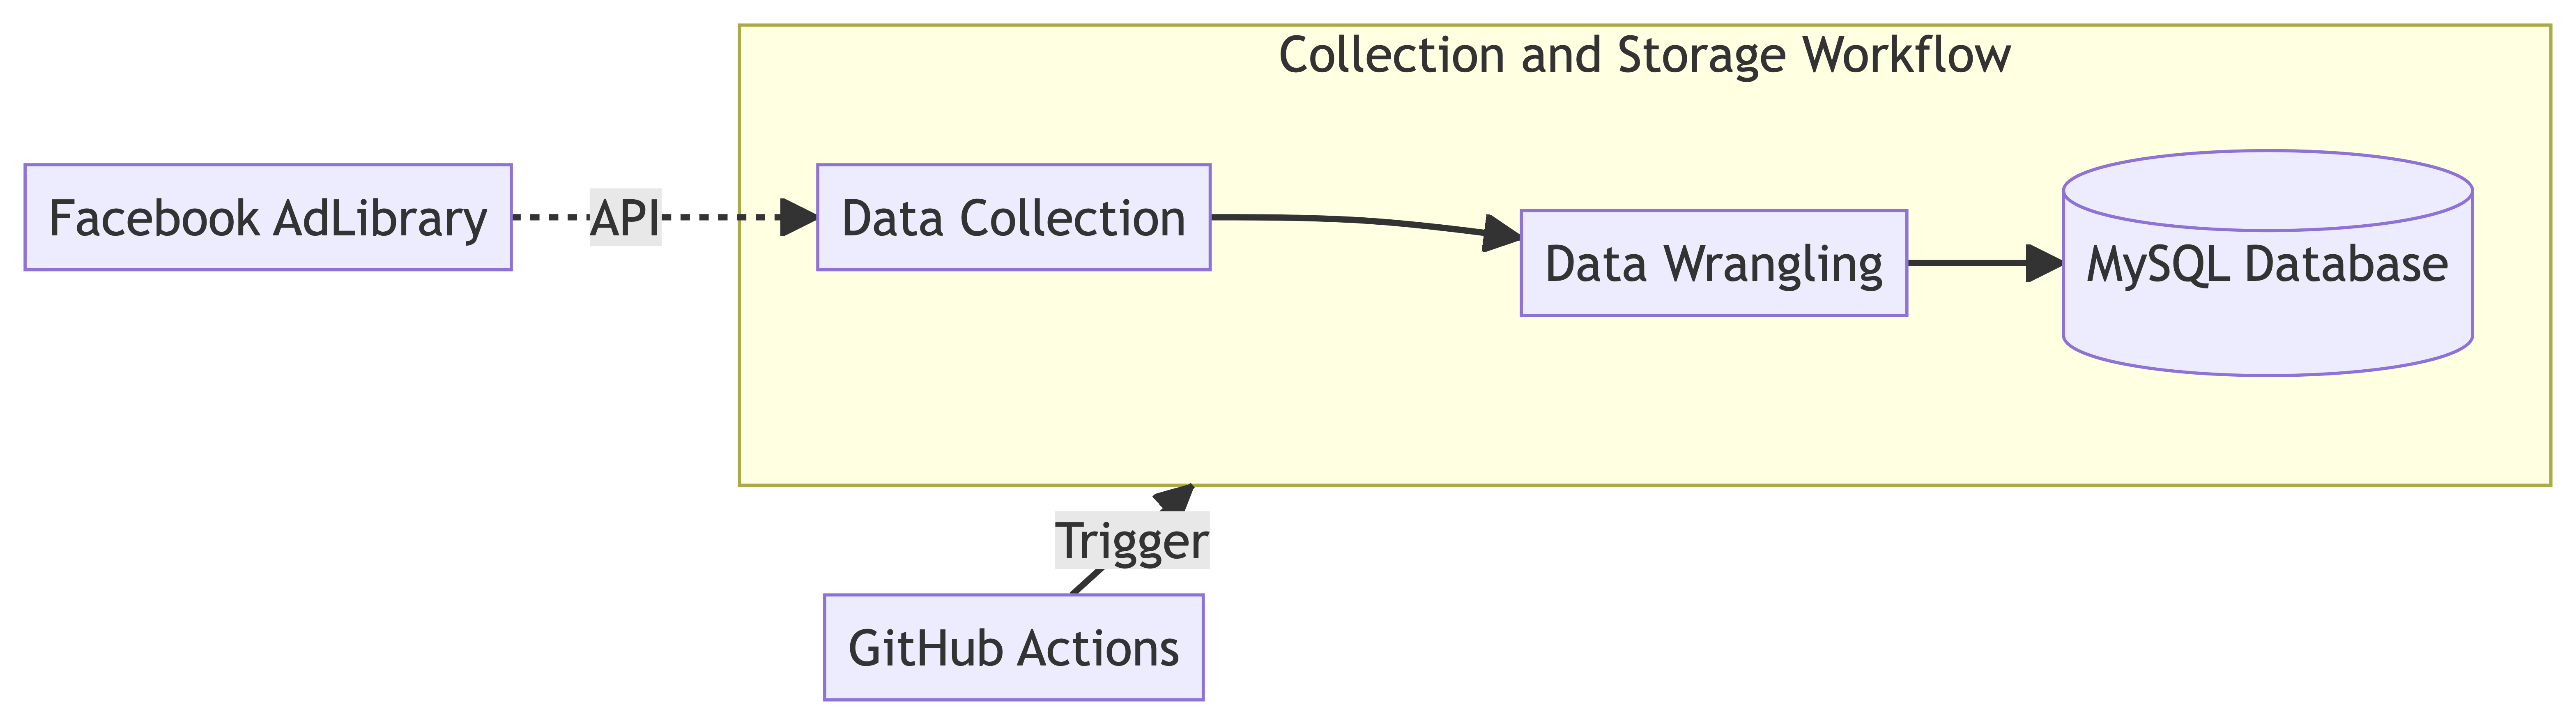
\includegraphics[width=8.57in,height=2.41in]{index_files/figure-latex/mermaid-figure-1.png}

\bookmarksetup{startatroot}

\chapter{Data collection}\label{sec-collection}

\section{Constructing our request}\label{constructing-our-request}

\subsection{Example request}\label{example-request}

To request data from Ad Library API when need to construct a request
url. Here is an example:

\begin{verbatim}
https://graph.facebook.com/v20.0/ads_archive?unmask_removed_content=true&ad_type=POLITICAL_AND_ISSUE_ADS&access_token=INSERT_YOUR_TOKEN&fields=id,ad_creation_time,ad_creative_bodies,ad_creative_link_captions,ad_creative_link_descriptions,ad_creative_link_titles,ad_delivery_start_time,ad_delivery_stop_time,ad_snapshot_url,currency,delivery_by_region,demographic_distribution,bylines,impressions,languages,page_id,page_name,publisher_platforms,spend,target_locations,target_gender,target_ages,estimated_audience_size&search_terms=.&ad_reached_countries=CA&search_page_ids=&ad_delivery_date_min=2020-05-22&ad_active_status=ALL&limit=500
\end{verbatim}

\textbf{Here are some of the key parameters of our request:}

\begin{itemize}
\item
  \texttt{limit=500}: request 500 ads at a time.
\item
  \texttt{ad\_delivery\_date\_min=2020-05-22}: only ads shown to users
  since 2020-05-22
\item
  \texttt{ad\_type=POLITICAL\_AND\_ISSUE\_ADS}: filter for only
  political ads
\item
  \texttt{unmask\_removed\_content=true}: include ads that broke
  Facebook's content guidelines
\item
  \texttt{ad\_active\_status=ALL}: ads don't have to be currently active
\item
  \texttt{ad\_reached\_countries=CA}: only ads shown in Canada
\end{itemize}

\subsection{How do we do this in our
code?}\label{how-do-we-do-this-in-our-code}

To construct the url dynamically based on the current date we adapted
some code provided by
\href{https://github.com/facebookresearch/Ad-Library-API-Script-Repository/tree/main}{Meta}.

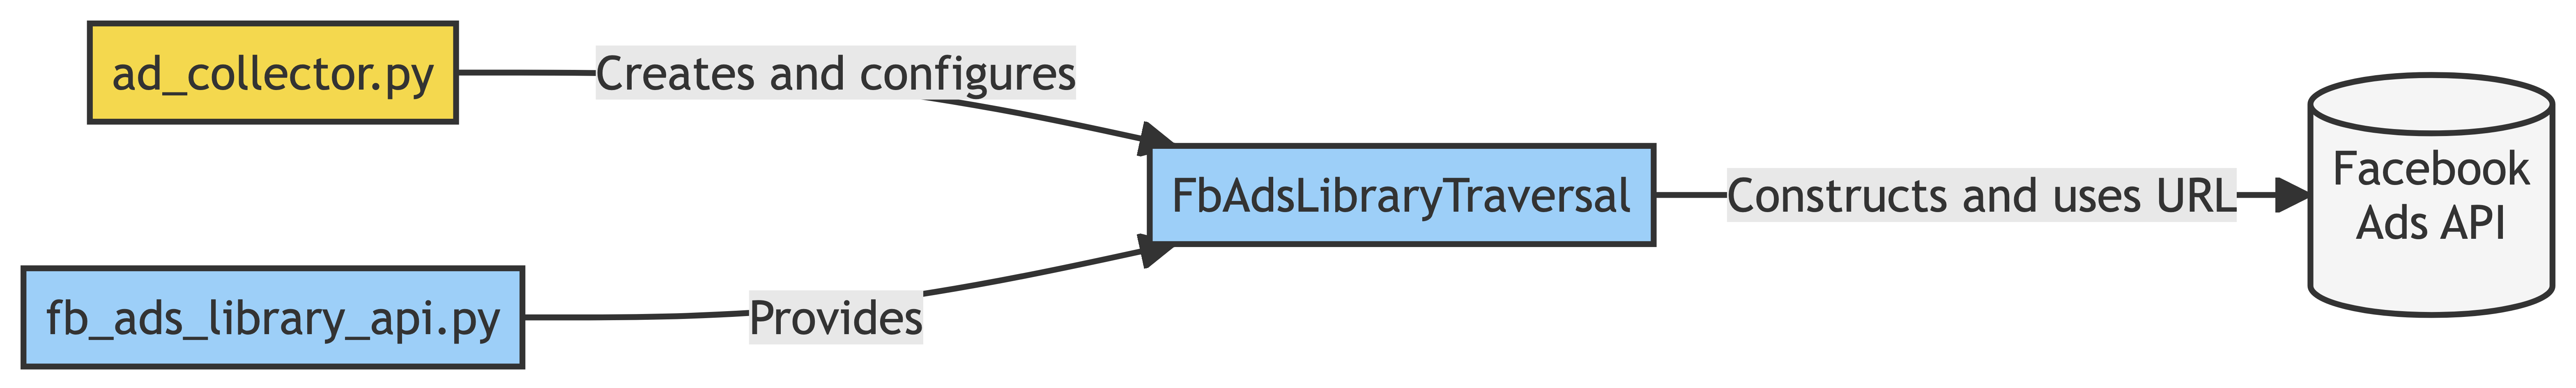
\includegraphics[width=9.16in,height=1.39in]{collection_files/figure-latex/mermaid-figure-1.png}

In \texttt{ad\_collector.py}, we use a class called
\texttt{FbAdsLibraryTraversal} from \texttt{fb\_ads\_library\_api.py}.
We then make an instance of this class with the details we need for our
API request.

Here is an example:

\begin{Shaded}
\begin{Highlighting}[]
\ImportTok{from}\NormalTok{ fb\_ads\_library\_api }\ImportTok{import}\NormalTok{ FbAdsLibraryTraversal}

\NormalTok{collector }\OperatorTok{=}\NormalTok{ FbAdsLibraryTraversal(}
\NormalTok{        facebook\_api\_keys,}
        \StringTok{"id,ad\_creation\_time,ad\_creative\_bodies,ad\_creative\_link\_captions,ad\_creative\_link\_descriptions,ad\_creative\_link\_titles,ad\_delivery\_start\_time,ad\_delivery\_stop\_time,ad\_snapshot\_url,currency,delivery\_by\_region,demographic\_distribution,bylines,impressions,languages,page\_id,page\_name,publisher\_platforms,spend,target\_locations,target\_gender,target\_ages,estimated\_audience\_size"}\NormalTok{,}
        \StringTok{"."}\NormalTok{,}
        \StringTok{"CA"}\NormalTok{,}
\NormalTok{        ad\_delivery\_date\_min}\OperatorTok{=}\NormalTok{start\_date,}
\NormalTok{        api\_version}\OperatorTok{=}\StringTok{"v20.0"}
\NormalTok{    )}
\end{Highlighting}
\end{Shaded}

Once our collector is set up, we make the API call using
\texttt{collector.generate\_ad\_archives()}. This returns a list of
dictionaries - one for each ad. The ads are returned in batches (of 500)
and we wrangle and extract the key details for submission to the
database.

\section{Avoiding API errors}\label{avoiding-api-errors}

\subsection{Too much data requested}\label{too-much-data-requested}

Some quarto are exceptionally long (\textasciitilde90,000 characters!).
This creates inconsistency around how many ads you can safely request at
once. To solve this we implement the following sliding window strategy:

\textbf{Step 1}: Start by collecting large number of ads (500)

\textbf{Step 2}: If we encounter ``Request less data'' error, halve
request size

\textbf{Step 3}: Repeat step 2 recursively

\textbf{Step 4}: If we successfully collect all 500, return to Step 1.
Otherwise, request problematic ad without body text.

\subsection{Too many requests made}\label{too-many-requests-made}

We use multiple API keys on rotation by creating multiple Meta `apps'.
This means that if one key reaches the limit \texttt{total\_time=100}
then we can switch to a different key.

\begin{tcolorbox}[enhanced jigsaw, breakable, colback=white, opacityback=0, bottomrule=.15mm, coltitle=black, bottomtitle=1mm, rightrule=.15mm, titlerule=0mm, colframe=quarto-callout-tip-color-frame, left=2mm, colbacktitle=quarto-callout-tip-color!10!white, opacitybacktitle=0.6, toptitle=1mm, title=\textcolor{quarto-callout-tip-color}{\faLightbulb}\hspace{0.5em}{Renewing API access}, arc=.35mm, leftrule=.75mm, toprule=.15mm]

Long term API tokens expire after three months so you have to renew
them.

\end{tcolorbox}

\section{Active vs launched ads}\label{active-vs-launched-ads}

\begin{tcolorbox}[enhanced jigsaw, breakable, colback=white, opacityback=0, bottomrule=.15mm, coltitle=black, bottomtitle=1mm, rightrule=.15mm, titlerule=0mm, colframe=quarto-callout-tip-color-frame, left=2mm, colbacktitle=quarto-callout-tip-color!10!white, opacitybacktitle=0.6, toptitle=1mm, title=\textcolor{quarto-callout-tip-color}{\faLightbulb}\hspace{0.5em}{Key distinction}, arc=.35mm, leftrule=.75mm, toprule=.15mm]

Meta's API only allows us to request the ads active during a date range,
not those launched. If you want launches, you can filter the data
afterwards. We submit all of the data to our database, without
filtering.

\end{tcolorbox}

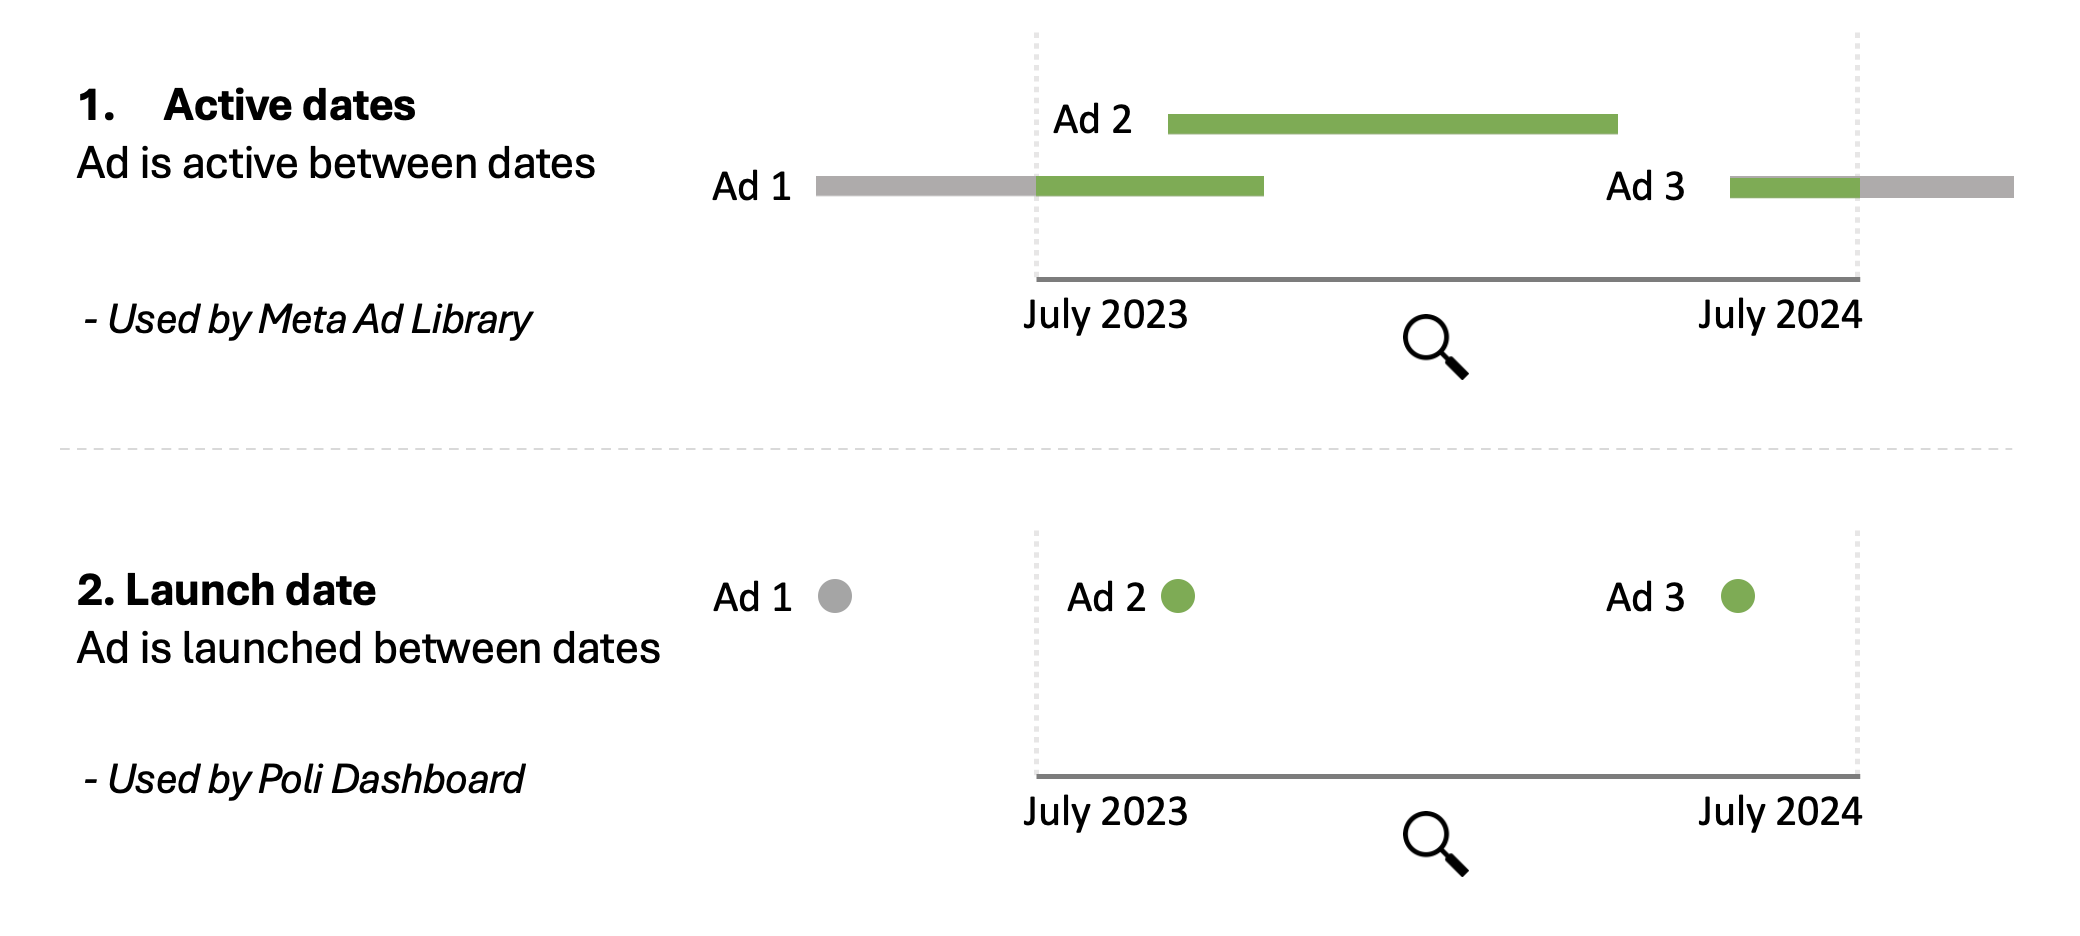
\includegraphics{img/active-launched.png}

\section{Daily data collection}\label{daily-data-collection}

\begin{itemize}
\item
  We use \textbf{Github Actions} to trigger the collection and storage
  of ads every day
\item
  At 12AM EST, we collect and update all ads active in the past month
\item
  At 8AM, 4PM and 8PM EST we collect and update all ads active on the
  current day
\end{itemize}

\bookmarksetup{startatroot}

\chapter{Data wrangling}\label{sec-wrangling}

\section{Diagram}\label{diagram}

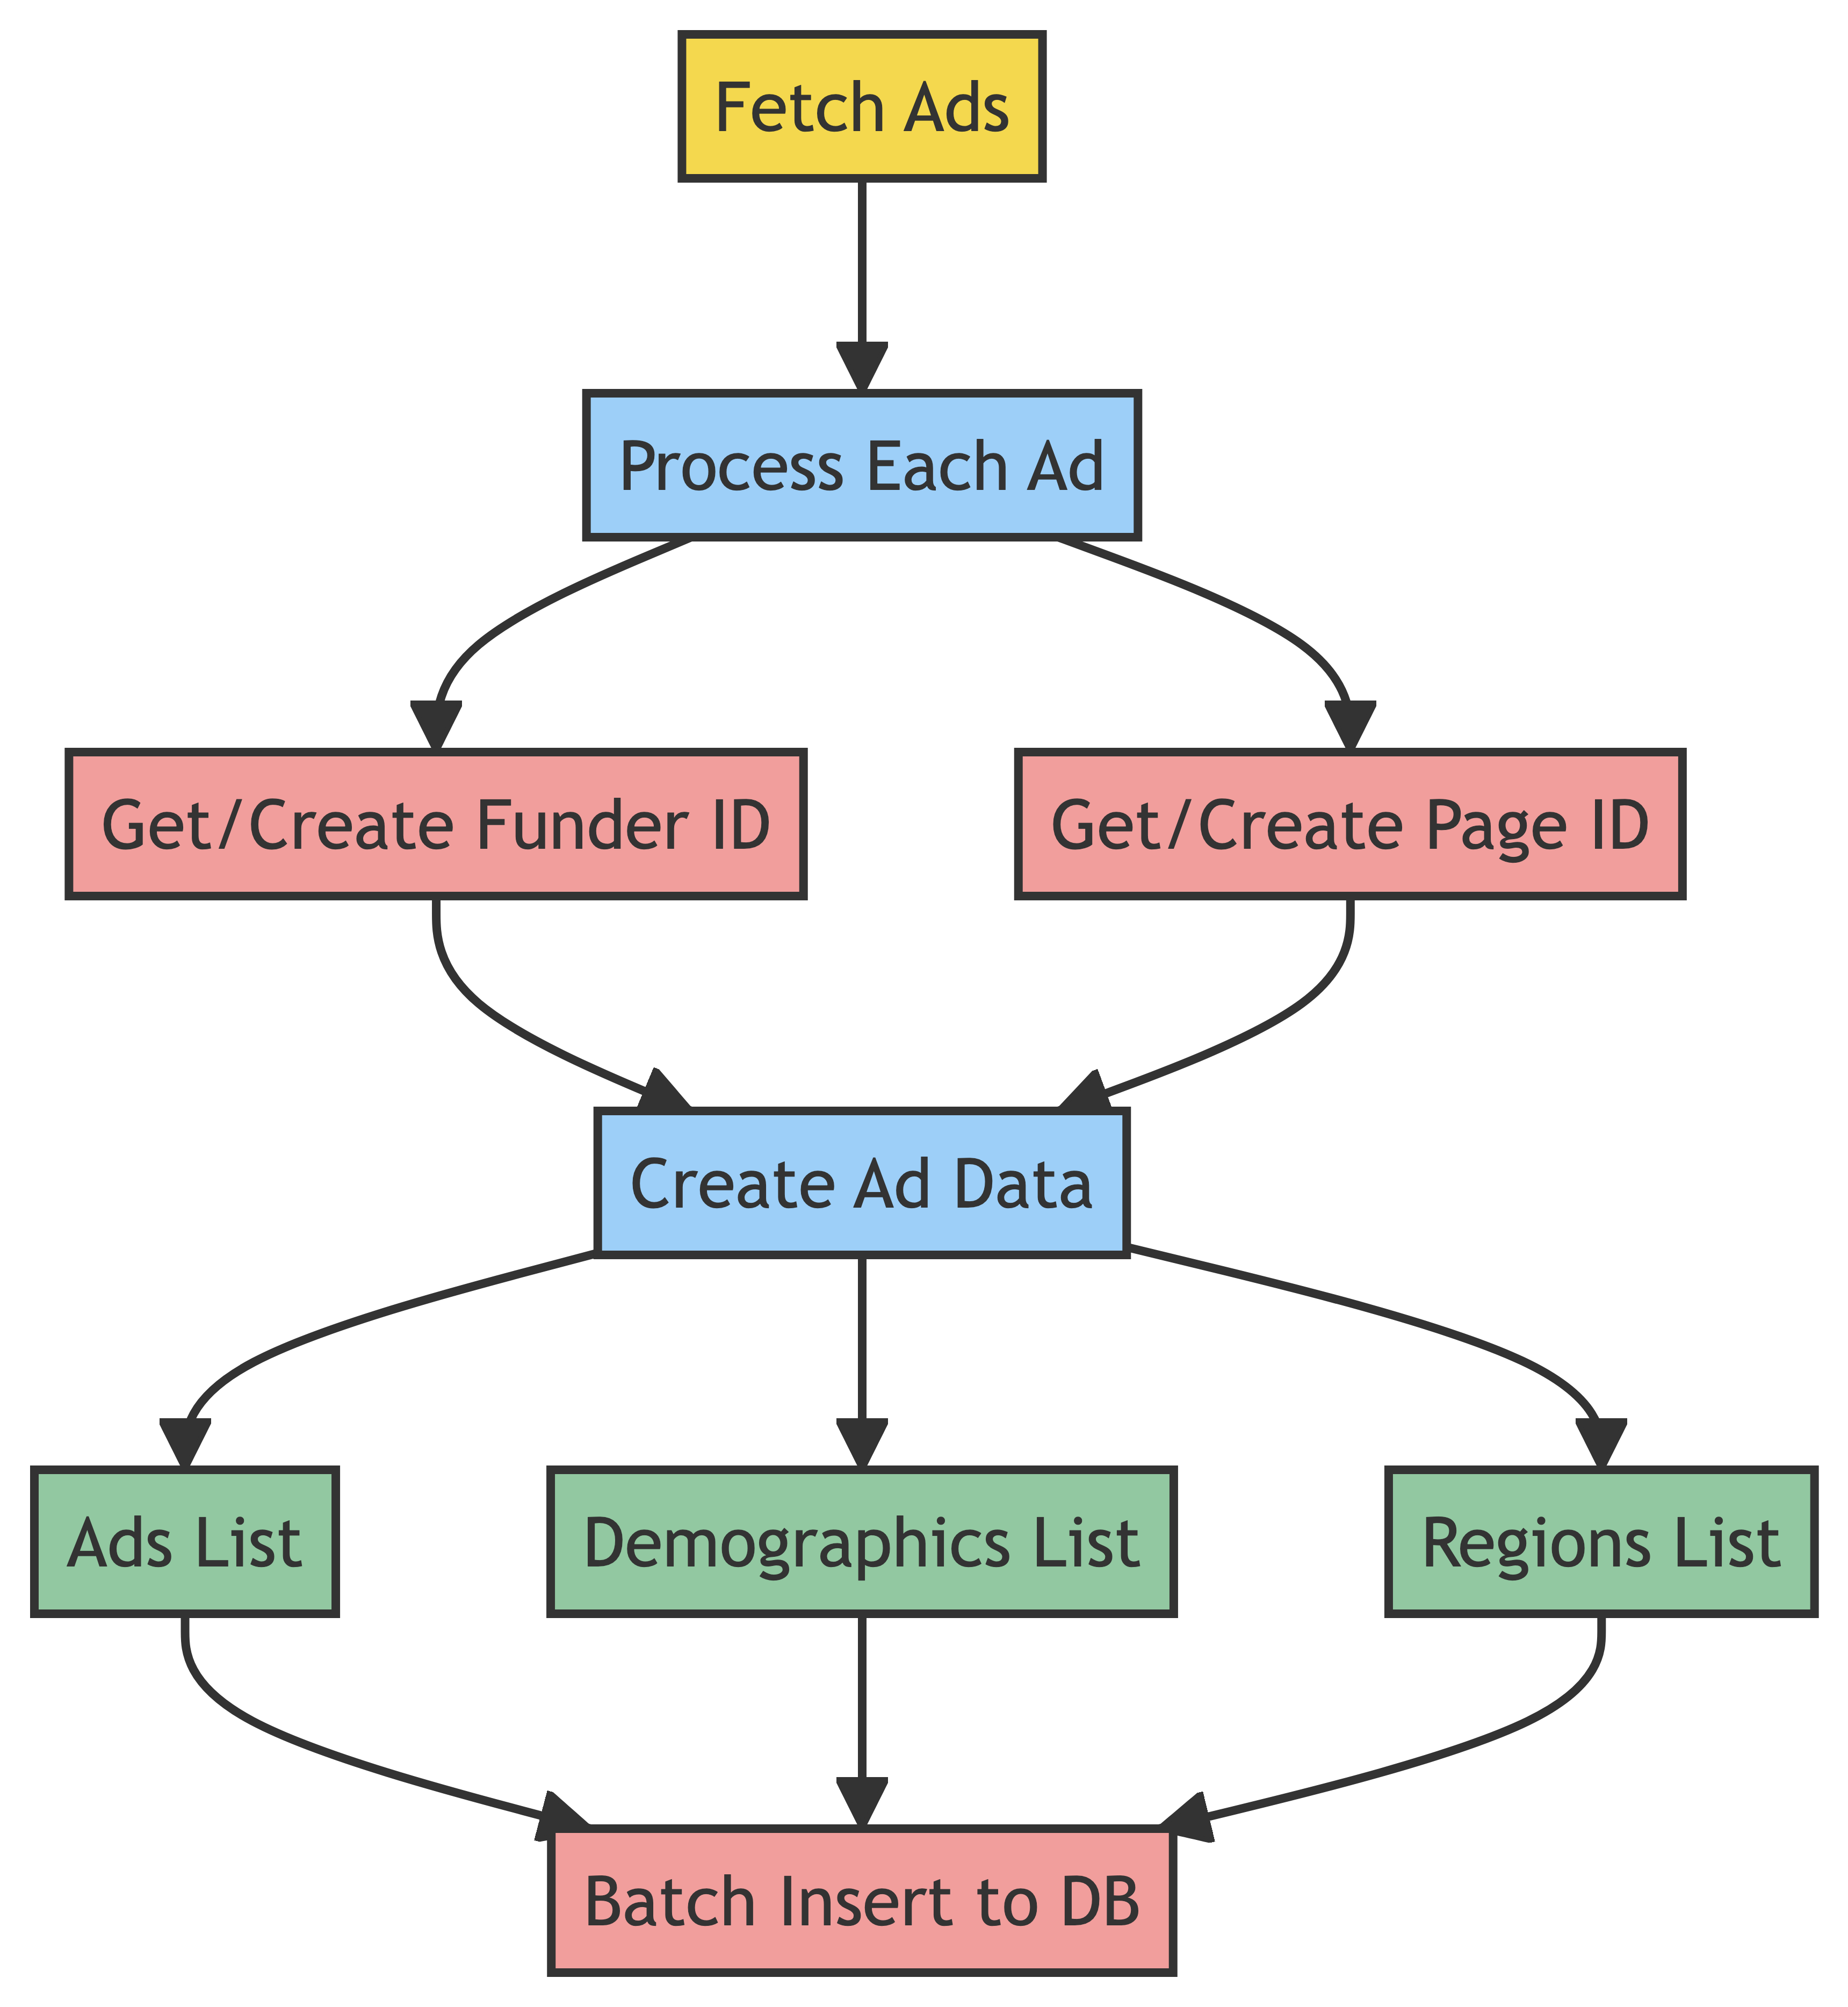
\includegraphics[width=4.48in,height=4.86in]{wrangling_files/figure-latex/mermaid-figure-1.png}

\section{Dealing with empty values}\label{dealing-with-empty-values}

Meta's API often returns ads with missing values, which can cause issues
with data integrity. Here is how we deal with each one:

\begin{longtable}[]{@{}
  >{\raggedright\arraybackslash}p{(\columnwidth - 2\tabcolsep) * \real{0.3509}}
  >{\raggedright\arraybackslash}p{(\columnwidth - 2\tabcolsep) * \real{0.6491}}@{}}
\toprule\noalign{}
\begin{minipage}[b]{\linewidth}\raggedright
Missing Field
\end{minipage} & \begin{minipage}[b]{\linewidth}\raggedright
Action Taken
\end{minipage} \\
\midrule\noalign{}
\endhead
\bottomrule\noalign{}
\endlastfoot
\texttt{page\_id} & Use a hashing algorithm to generate one based on the
page name. Derived ids are tracked by the \texttt{is\_derived} property
in the pages table. \\
\texttt{end\_date} & Use the current date and store ongoing status in a
boolean \texttt{is\_active} \\
\texttt{estimated\_audience\_size} or \texttt{impressions} upper bound &
Set equal to lower bound \\
\texttt{gender} or \texttt{age} & Set as `unspecified' \\
\end{longtable}

\section{Dealing with non-Canadian
adverts}\label{dealing-with-non-canadian-adverts}

Often, advertisers based outside of Canada will include users within
Canada for a very small fraction of their ad targeting. For
comprehensiveness, we opted to collect these ads. However, any
non-Canadian regions are aggregated as `Overseas' in our database.

\section{Property names}\label{property-names}

Here is a translation of Meta's API properties to our own database:

\begin{longtable}[]{@{}
  >{\raggedright\arraybackslash}p{(\columnwidth - 2\tabcolsep) * \real{0.5278}}
  >{\raggedright\arraybackslash}p{(\columnwidth - 2\tabcolsep) * \real{0.4722}}@{}}
\toprule\noalign{}
\begin{minipage}[b]{\linewidth}\raggedright
Meta API Property
\end{minipage} & \begin{minipage}[b]{\linewidth}\raggedright
Our Database Field
\end{minipage} \\
\midrule\noalign{}
\endhead
\bottomrule\noalign{}
\endlastfoot
\texttt{id} & \texttt{id} \\
\texttt{page\_id} & \texttt{page\_id} \\
\texttt{funder\_id} & \texttt{funder\_id} \\
\texttt{ad\_creation\_time} & \texttt{created\_date} \\
\texttt{ad\_delivery\_start\_time} & \texttt{start\_date} \\
\texttt{ad\_delivery\_stop\_time} & \texttt{end\_date} \\
& \texttt{is\_active} \\
\texttt{ad\_snapshot\_url} & \texttt{ad\_library\_url} \\
\texttt{currency} & \texttt{currency} \\
\texttt{estimated\_audience\_size.lower\_bound} &
\texttt{audience\_min} \\
\texttt{estimated\_audience\_size.upper\_bound} &
\texttt{audience\_max} \\
\texttt{impressions.lower\_bound} & \texttt{views\_min} \\
\texttt{impressions.upper\_bound} & \texttt{views\_max} \\
\texttt{spend.lower\_bound} & \texttt{cost\_min} \\
\texttt{spend.upper\_bound} & \texttt{cost\_max} \\
\texttt{publisher\_platforms} & \texttt{platforms} \\
\texttt{languages} & \texttt{languages} \\
\texttt{ad\_creative\_bodies} & \texttt{body} \\
\texttt{ad\_creative\_link\_captions} & \texttt{link\_url} \\
\texttt{ad\_creative\_link\_descriptions} & \texttt{description} \\
\texttt{ad\_creative\_link\_titles} & \texttt{link\_title} \\
\texttt{delivery\_by\_region} & \texttt{provinces} \\
\texttt{demographic\_distribution} & \texttt{demographics} \\
\end{longtable}

\bookmarksetup{startatroot}

\chapter{MySQL database}\label{sec-database}

\section{Core database tables}\label{core-database-tables}

Our MySQL database comprises five tables. The \texttt{ads} table is
linked by \texttt{page\_id} and \texttt{funder\_id} to the
\texttt{pages} and \texttt{funders} tables. Each ad in the \texttt{ads}
table is linked to the \texttt{ad\_demographics} and
\texttt{ad\_provinces} tables.

Here is the basic setup:

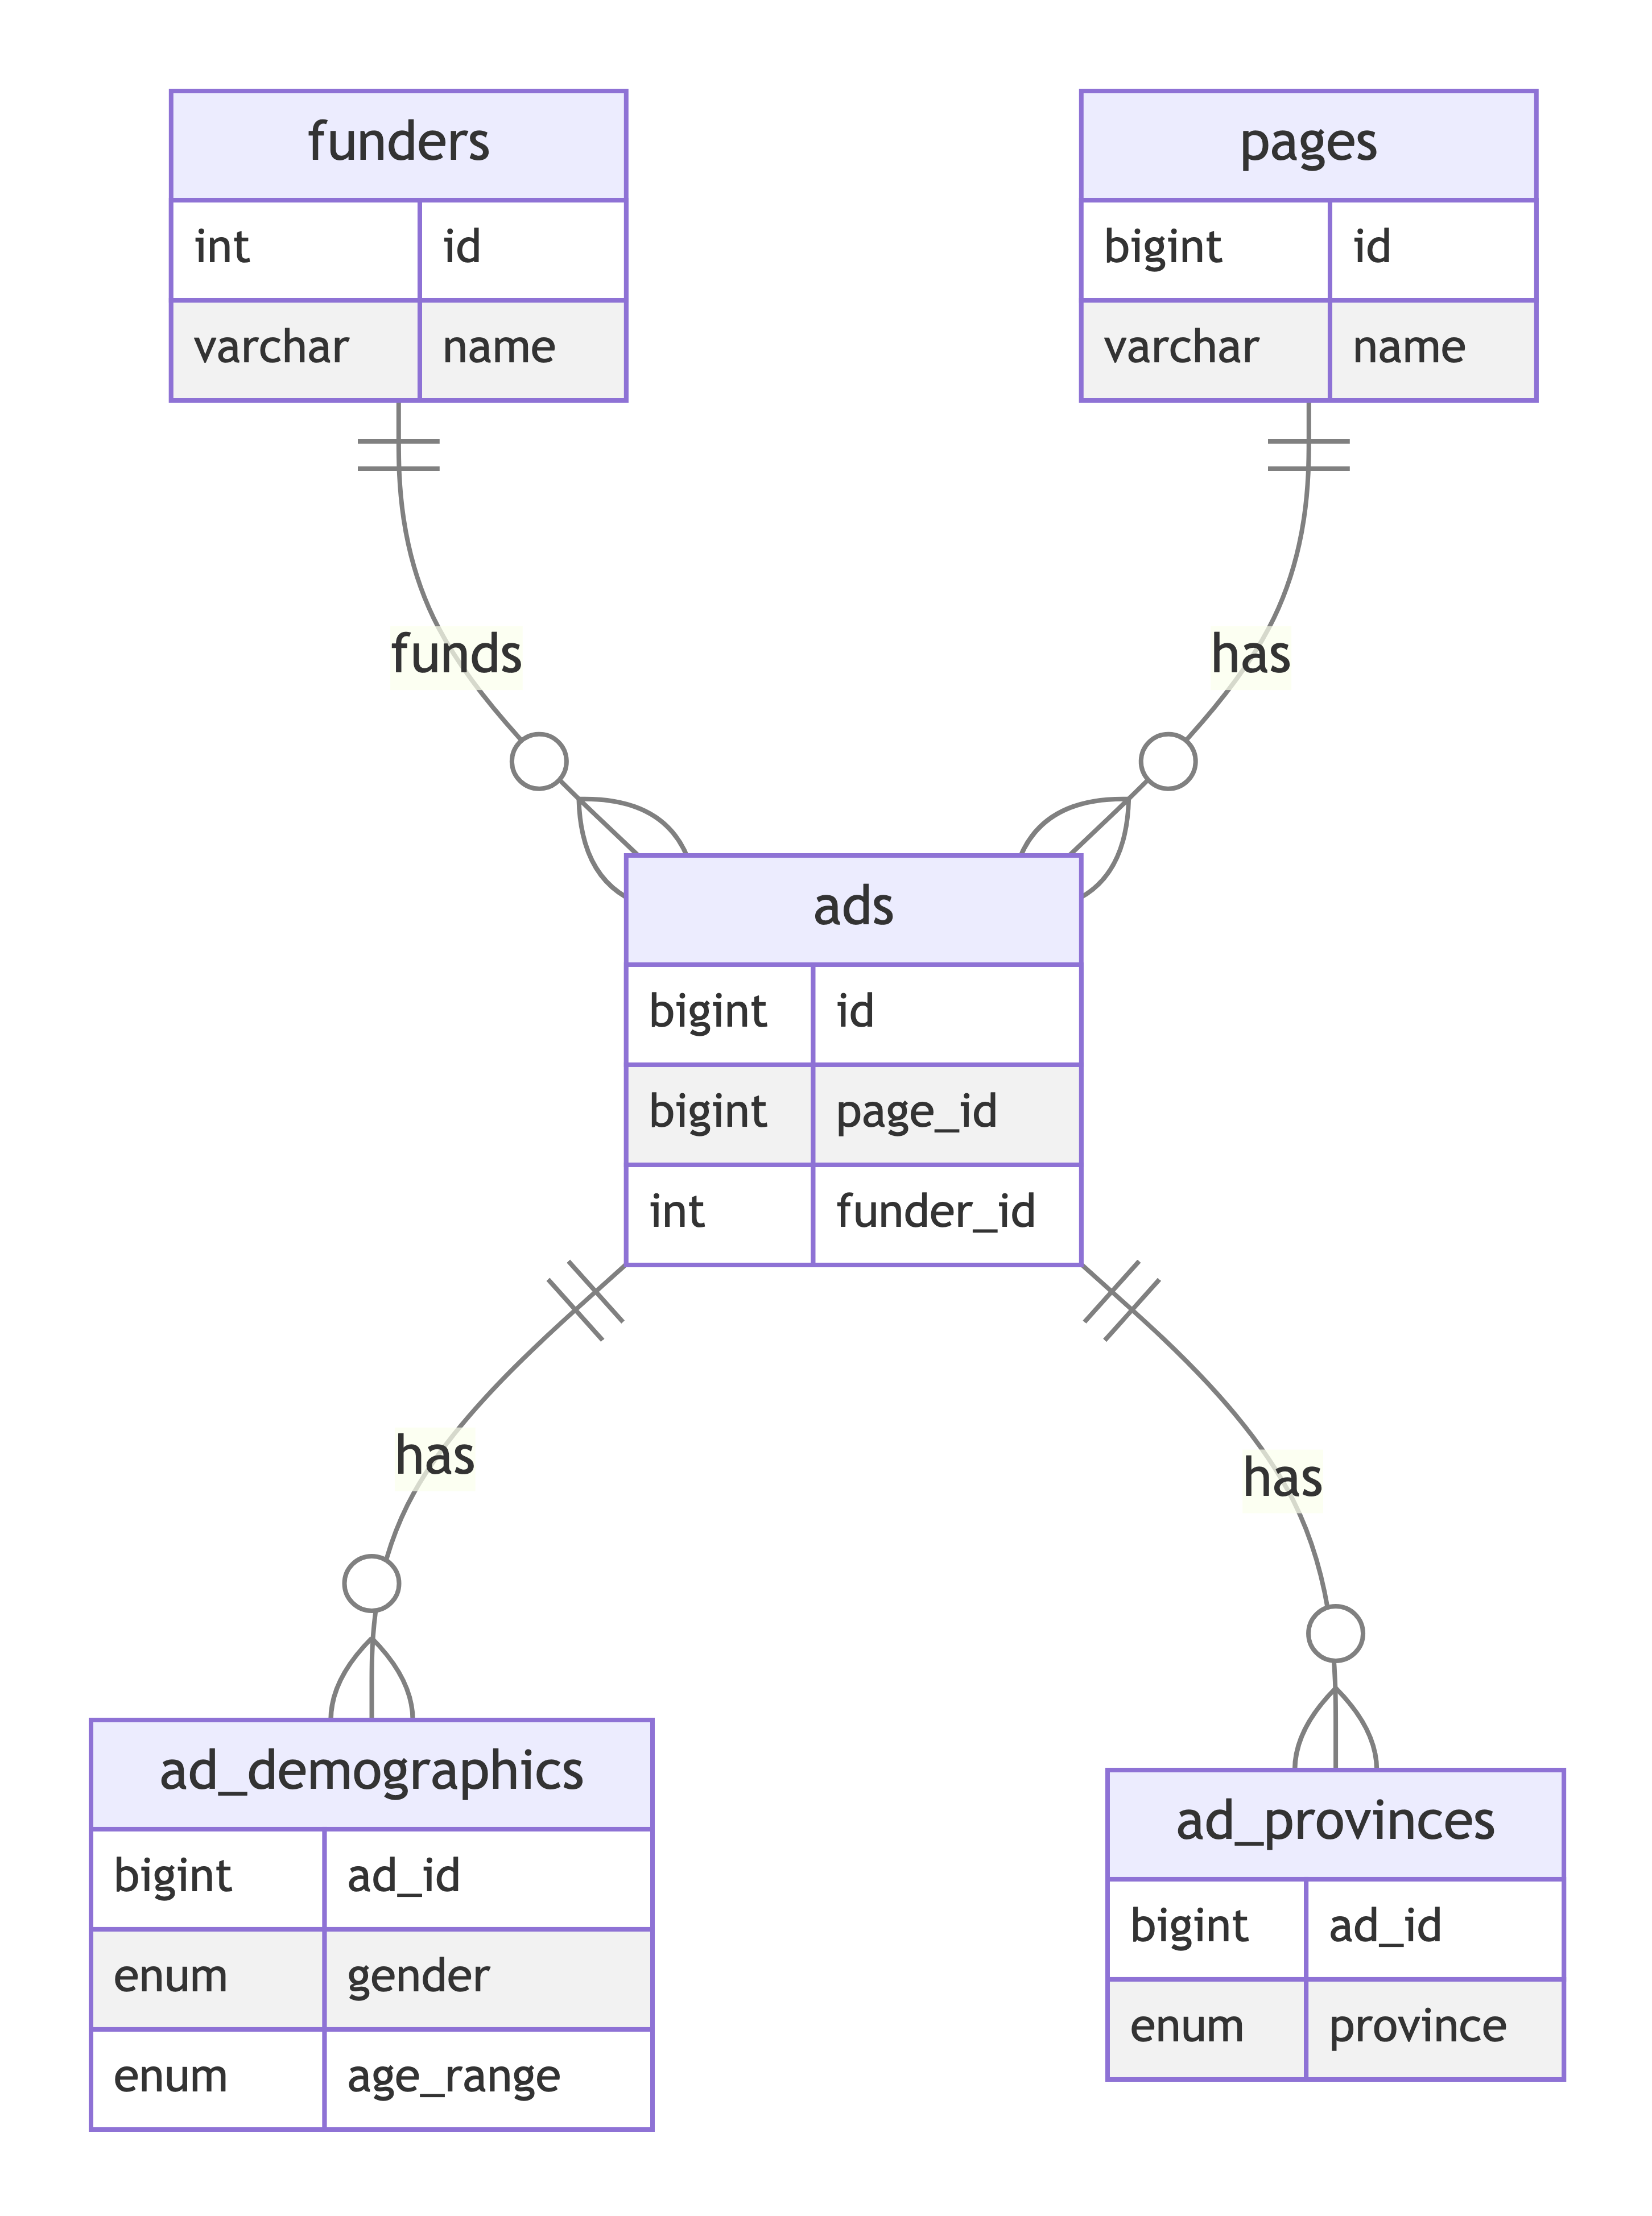
\includegraphics[width=6in,height=8.05in]{database_files/figure-latex/mermaid-figure-1.png}

\section{Simplifying querying}\label{simplifying-querying}

Writing useful queries often involves joining many tables together and
can be cumbersome for quick data analysis. We have designed
\texttt{VIEWS} and \texttt{PROCEDURES} that make it easier to see
interesting results.

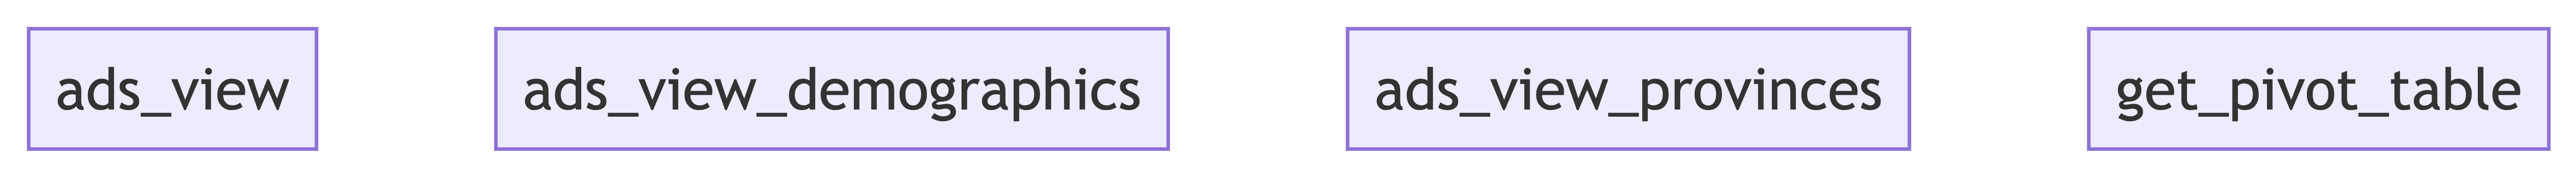
\includegraphics[width=7.48in,height=0.52in]{database_files/figure-latex/mermaid-figure-2.png}

\subsection{Views}\label{views}

\begin{longtable}[]{@{}
  >{\raggedright\arraybackslash}p{(\columnwidth - 4\tabcolsep) * \real{0.1004}}
  >{\raggedright\arraybackslash}p{(\columnwidth - 4\tabcolsep) * \real{0.4100}}
  >{\raggedright\arraybackslash}p{(\columnwidth - 4\tabcolsep) * \real{0.4895}}@{}}
\toprule\noalign{}
\begin{minipage}[b]{\linewidth}\raggedright
View Name
\end{minipage} & \begin{minipage}[b]{\linewidth}\raggedright
Description
\end{minipage} & \begin{minipage}[b]{\linewidth}\raggedright
Example Query
\end{minipage} \\
\midrule\noalign{}
\endhead
\bottomrule\noalign{}
\endlastfoot
\texttt{ads\_view} & Returns one row per advert, including
\texttt{funder\_name} and \texttt{page\_name} for simpler querying. &
\texttt{SELECT\ *\ FROM\ ads\_view\ WHERE\ funder\_name\ =\ \textquotesingle{}Conservative\ Party\ of\ Canada\ -\ Parti\ conservateur\ du\ Canada\textquotesingle{}\ AND\ start\_date\ \textgreater{}\ \textquotesingle{}2024-07-01\textquotesingle{};} \\
\texttt{ads\_view\_demographics} & Returns multiple rows per advert: one
for each demographic targeted. &
\texttt{SELECT\ *\ FROM\ ads\_view\_demographics\ WHERE...} \\
\texttt{ads\_view\_provinces} & Returns multiple rows per advert: one
for each province targeted. &
\texttt{SELECT\ *\ FROM\ ads\_view\_provinces\ WHERE...} \\
\end{longtable}

\subsection{Pivot tables}\label{sec-pivot}

The \texttt{get\_pivot\_table} stored procedure allows you to generate a
pivot table that aggregates data about ads based on specific criteria.

\begin{Shaded}
\begin{Highlighting}[]
\KeywordTok{CALL}\NormalTok{ get\_pivot\_table(}\StringTok{\textquotesingle{}"climate change"\textquotesingle{}}\NormalTok{, }\StringTok{\textquotesingle{}2024{-}06{-}01\textquotesingle{}}\NormalTok{, }\StringTok{\textquotesingle{}2024{-}06{-}30\textquotesingle{}}\NormalTok{, }\StringTok{\textquotesingle{}funder\textquotesingle{}}\NormalTok{)}
\end{Highlighting}
\end{Shaded}

The procedure takes the following parameters:

\begin{itemize}
\tightlist
\item
  \textbf{p\_keyword} (VARCHAR): A keyword to filter ads by their
  content, description, and link title. If \texttt{NULL}, no keyword
  filter is applied.
\item
  \textbf{p\_start\_date} (DATE): The start date of the period for which
  data is to be aggregated.
\item
  \textbf{p\_end\_date} (DATE): The end date of the period for which
  data is to be aggregated.
\item
  \textbf{p\_group\_by} (VARCHAR): The dimension by which to group the
  results. Can be \texttt{funder}, \texttt{page}, or \texttt{both}
  (default).
\end{itemize}

This aggregates spending and views for each entity based on ads active
in the period. For more information on how this is calculated see
Section~\ref{sec-spending}.

\section{Table properties}\label{table-properties}

Select a table to view its properties.

\subsection{funders}

\begin{longtable}[]{@{}l@{}}
\toprule\noalign{}
Property \\
\midrule\noalign{}
\endhead
\bottomrule\noalign{}
\endlastfoot
id \\
name \\
\end{longtable}

\subsection{pages}

\begin{longtable}[]{@{}l@{}}
\toprule\noalign{}
Property \\
\midrule\noalign{}
\endhead
\bottomrule\noalign{}
\endlastfoot
id \\
name \\
is\_derived\_id \\
\end{longtable}

\subsection{ads}

\begin{longtable}[]{@{}l@{}}
\toprule\noalign{}
Property \\
\midrule\noalign{}
\endhead
\bottomrule\noalign{}
\endlastfoot
id \\
page\_id \\
funder\_id \\
created\_date \\
start\_date \\
end\_date \\
is\_active \\
ad\_library\_url \\
currency \\
audience\_min \\
audience\_max \\
views\_min \\
views\_max \\
cost\_min \\
cost\_max \\
content\_id \\
platforms \\
languages \\
body \\
link\_url \\
description \\
link\_title \\
provinces \\
demographics \\
\end{longtable}

\subsection{ad\_demographics}

\begin{longtable}[]{@{}l@{}}
\toprule\noalign{}
Property \\
\midrule\noalign{}
\endhead
\bottomrule\noalign{}
\endlastfoot
ad\_id \\
gender \\
age\_range \\
age\_gender\_percentage \\
\end{longtable}

\subsection{ad\_provinces}

\begin{longtable}[]{@{}l@{}}
\toprule\noalign{}
Property \\
\midrule\noalign{}
\endhead
\bottomrule\noalign{}
\endlastfoot
ad\_id \\
province \\
province\_percentage \\
\end{longtable}

\subsection{ads\_view}

\begin{longtable}[]{@{}l@{}}
\toprule\noalign{}
Property \\
\midrule\noalign{}
\endhead
\bottomrule\noalign{}
\endlastfoot
ad\_id \\
page\_id \\
page\_name \\
funder\_name \\
start\_date \\
end\_date \\
is\_active \\
ad\_library\_url \\
currency \\
views\_min \\
views\_max \\
cost\_min \\
cost\_max \\
platforms \\
languages \\
body \\
link\_url \\
description \\
link\_title \\
provinces \\
demographics \\
\end{longtable}

\subsection{ads\_view\_demographics}

\begin{longtable}[]{@{}l@{}}
\toprule\noalign{}
Property \\
\midrule\noalign{}
\endhead
\bottomrule\noalign{}
\endlastfoot
ad\_id \\
page\_name \\
funder\_name \\
start\_date \\
end\_date \\
is\_active \\
ad\_library\_url \\
currency \\
views\_min \\
views\_max \\
cost\_min \\
cost\_max \\
platforms \\
languages \\
body \\
link\_url \\
description \\
link\_title \\
gender \\
age\_range \\
age\_gender\_percentage \\
\end{longtable}

\subsection{ads\_view\_provinces}

\begin{longtable}[]{@{}l@{}}
\toprule\noalign{}
Property \\
\midrule\noalign{}
\endhead
\bottomrule\noalign{}
\endlastfoot
ad\_id \\
page\_name \\
funder\_name \\
start\_date \\
end\_date \\
is\_active \\
ad\_library\_url \\
currency \\
views\_min \\
views\_max \\
cost\_min \\
cost\_max \\
platforms \\
languages \\
body \\
link\_url \\
description \\
link\_title \\
province \\
province\_percentage \\
\end{longtable}

\subsection{get\_pivot\_table}

\begin{longtable}[]{@{}l@{}}
\toprule\noalign{}
Property \\
\midrule\noalign{}
\endhead
\bottomrule\noalign{}
\endlastfoot
group\_id \\
group\_name \\
ad\_count \\
total\_min\_spend\_for\_period \\
total\_max\_spend\_for\_period \\
total\_min\_views\_for\_period \\
total\_max\_views\_for\_period \\
\end{longtable}

\section{Top Tips for Querying}\label{top-tips-for-querying}

\begin{enumerate}
\def\labelenumi{\arabic{enumi}.}
\item
  Include both the \texttt{start\_date} and \texttt{end\_date}
  properties as the query will be faster than filtering by just one.
\item
  For most queries, use the \texttt{ads\_view} table rather than
  \texttt{ads}. It's faster even for counting rows.
\item
  If the database is slow, try to restrict your search. E.g. use a
  \texttt{WHERE} clause to search for a specific funder, keyword, date
  range combination.
\item
  Avoid trying to join unparsed demographic, regional and ad together
  together as you get row explosion.
\item
  There are two different strategies for filtering by date:
\end{enumerate}

\chapter{Querying by active date}

\begin{Shaded}
\begin{Highlighting}[]
\NormalTok{end\_date }\OperatorTok{\textgreater{}=} \DecValTok{2024}\OperatorTok{{-}}\DecValTok{01}\OperatorTok{{-}}\DecValTok{01} \KeywordTok{and}\NormalTok{ start\_date }\OperatorTok{\textless{}=} \DecValTok{2024}\OperatorTok{{-}}\DecValTok{01}\OperatorTok{{-}}\DecValTok{31}
\end{Highlighting}
\end{Shaded}

Returns all ads active in January 2024. This is the method used by the
Facebook Ad Library and report.

\chapter{Querying by launch date}

\begin{Shaded}
\begin{Highlighting}[]
\NormalTok{start\_date }\OperatorTok{\textgreater{}=} \DecValTok{2024}\OperatorTok{{-}}\DecValTok{01}\OperatorTok{{-}}\DecValTok{01} \KeywordTok{and}\NormalTok{ start\_date }\OperatorTok{\textless{}=} \DecValTok{2024}\OperatorTok{{-}}\DecValTok{01}\OperatorTok{{-}}\DecValTok{31}
\end{Highlighting}
\end{Shaded}

Returns all ads launched in January 2024.

\bookmarksetup{startatroot}

\chapter{Query Library}\label{sec-library}

Discover useful queries.

\begin{verbatim}
<IPython.core.display.HTML object>
\end{verbatim}

\begin{Shaded}
\begin{Highlighting}[]
\NormalTok{\{}
\NormalTok{  const queries = \{\};}

\NormalTok{// Transform the original object}
\NormalTok{    data.Name.forEach((name, index) =\textgreater{} \{}
\NormalTok{    queries[name] = \{}
\NormalTok{        query: data.Query[index],}
\NormalTok{        note: data.Notes[index]}
\NormalTok{    \};}
\NormalTok{    \});}

\NormalTok{  const styles = html\textasciigrave{}\textless{}style\textgreater{}}
\NormalTok{    \#container \{}
\NormalTok{      display: flex;}
\NormalTok{      height: 400px;}
\NormalTok{      background: \#101b3d;}
\NormalTok{      font{-}family: sans{-}serif;}
\NormalTok{    \}}
\NormalTok{    \#sidebar \{}
\NormalTok{      width: 30\%;}
\NormalTok{      padding: 20px;}
\NormalTok{      box{-}sizing: border{-}box;}
\NormalTok{      display: flex;}
\NormalTok{      flex{-}direction: column;}
\NormalTok{      height: 400px;}
\NormalTok{      color: \#8892b0;}
\NormalTok{      font{-}size: 0.85rem;}
\NormalTok{      font{-}weight: bold;}
\NormalTok{    \}}
\NormalTok{    \#search{-}box \{}
\NormalTok{      width: 100\%;}
\NormalTok{      padding: 10px;}
\NormalTok{      margin{-}bottom: 10px;}
\NormalTok{      border: 1px solid \#233554; }
\NormalTok{      border{-}radius: 5px;}
\NormalTok{      color: \#8892b0;}
\NormalTok{      background{-}color: \#172a45;}
\NormalTok{    \}}
\NormalTok{    \#query{-}list \{}
\NormalTok{      flex{-}grow: 1;}
\NormalTok{      overflow{-}y: auto;}
\NormalTok{      border: 1px solid \#233554;}
\NormalTok{      border{-}radius: 5px;}
\NormalTok{      max{-}height: calc(100vh {-} 100px);}
\NormalTok{      background{-}color: \#172a45;}
\NormalTok{    \}}
\NormalTok{    .query{-}option \{}
\NormalTok{      padding: 10px;}
\NormalTok{      cursor: pointer;}
\NormalTok{      transition: background{-}color 0.3s;}
\NormalTok{      border{-}bottom: 1px solid \#233554;}
\NormalTok{    \}}
\NormalTok{    .query{-}option:hover \{}
\NormalTok{      background{-}color: \#1d3456;}
\NormalTok{    \}}
\NormalTok{    \#content \{}
\NormalTok{      width: 70\%;}
\NormalTok{      padding: 20px;}
\NormalTok{      box{-}sizing: border{-}box;}
\NormalTok{      display: flex;}
\NormalTok{      flex{-}direction: column;}
\NormalTok{      height: 400px;}
\NormalTok{    \}}
\NormalTok{    \#query{-}editor \{}
\NormalTok{      width: 100\%;}
\NormalTok{      flex{-}grow: 1;}
\NormalTok{      font{-}family: \textquotesingle{}Courier New\textquotesingle{}, monospace;}
\NormalTok{      padding: 20px;}
\NormalTok{      border: 1px solid \#233554;}
\NormalTok{      border{-}radius: 5px;}
\NormalTok{      font{-}size: 18px;}
\NormalTok{      line{-}height: 1.5;}
\NormalTok{      background{-}color: \#172a45;}
\NormalTok{      color: \#8892b0;}
\NormalTok{      box{-}shadow: inset 0 0 10px rgba(0,0,0,0.1);}
\NormalTok{      overflow{-}y: auto;}
\NormalTok{      white{-}space: pre{-}wrap;}
\NormalTok{      word{-}wrap: break{-}word;}
\NormalTok{    \}}
\NormalTok{    \#query{-}editor:focus \{}
\NormalTok{      outline: none;}
\NormalTok{    \}}
\NormalTok{    \#query{-}note \{}
\NormalTok{      margin{-}top: 10px;}
\NormalTok{      padding: 10px;}
\NormalTok{      background{-}color: \#233554;}
\NormalTok{      border{-}radius: 5px;}
\NormalTok{      color: \#8892b0;}
\NormalTok{      font{-}size: 0.9rem;}
\NormalTok{    \}}
\NormalTok{    .keyword \{ color: \#ff79c6; \}}
\NormalTok{    .function \{ color: \#8be9fd; \}}
\NormalTok{    .string \{ color: \#f1fa8c; \}}
\NormalTok{    .number \{ color: \#bd93f9; \}}
\NormalTok{    .comment \{ color: \#6272a4; \}}
\NormalTok{  \textless{}/style\textgreater{}\textasciigrave{};}

\NormalTok{  const container = html\textasciigrave{}\textless{}div id="container"\textgreater{}\textasciigrave{};}
  
\NormalTok{  const sidebar = html\textasciigrave{}\textless{}div id="sidebar"\textgreater{}\textasciigrave{};}
\NormalTok{  const searchBox = html\textasciigrave{}\textless{}input type="text" id="search{-}box" placeholder="Search queries..."\textgreater{}\textasciigrave{};}
\NormalTok{  const queryList = html\textasciigrave{}\textless{}div id="query{-}list"\textgreater{}\textasciigrave{};}

\NormalTok{  const content = html\textasciigrave{}\textless{}div id="content"\textgreater{}\textasciigrave{};}
\NormalTok{  const queryEditor = html\textasciigrave{}\textless{}div id="query{-}editor" contenteditable="true" spellcheck="false"\textgreater{}\textless{}/div\textgreater{}\textasciigrave{};}
\NormalTok{  const queryNote = html\textasciigrave{}\textless{}div id="query{-}note"\textgreater{}\textless{}/div\textgreater{}\textasciigrave{};}

\NormalTok{  function renderQueryList(filter = \textquotesingle{}\textquotesingle{}) \{}
\NormalTok{    queryList.innerHTML = \textquotesingle{}\textquotesingle{};  }
\NormalTok{    Object.keys(queries).forEach(key =\textgreater{} \{}
\NormalTok{      if (key.toLowerCase().includes(filter.toLowerCase())) \{}
\NormalTok{        const option = html\textasciigrave{}\textless{}div class="query{-}option"\textgreater{}$\{key\}\textless{}/div\textgreater{}\textasciigrave{};}
\NormalTok{        option.onclick = () =\textgreater{} \{}
\NormalTok{          queryEditor.textContent = queries[key].query;}
\NormalTok{          queryNote.textContent = queries[key].note;}
\NormalTok{          highlightSyntax();}
\NormalTok{        \};}
\NormalTok{        queryList.appendChild(option);}
\NormalTok{      \}}
\NormalTok{    \}); }
\NormalTok{  \}}

\NormalTok{  function highlightSyntax() \{}
\NormalTok{    let text = queryEditor.innerText;}
\NormalTok{    text = text.replace(/\textbackslash{}b(CALL|SELECT|FROM|WHERE|JOIN|ON|GROUP BY|HAVING|ORDER BY|UNION|CASE|WHEN|THEN|ELSE|END|AS|WITH)\textbackslash{}b/gi, \textquotesingle{}\textless{}span class="keyword"\textgreater{}$1\textless{}/span\textgreater{}\textquotesingle{});}
\NormalTok{    text = text.replace(/\textbackslash{}b(AVG|SUM|COUNT|MAX|MIN)\textbackslash{}b/gi, \textquotesingle{}\textless{}span class="function"\textgreater{}$1\textless{}/span\textgreater{}\textquotesingle{});}
\NormalTok{    text = text.replace(/\textquotesingle{}([\^{}\textquotesingle{}]*)\textquotesingle{}/g, \textquotesingle{}\textless{}span class="string"\textgreater{}\textbackslash{}\textquotesingle{}$1\textbackslash{}\textquotesingle{}\textless{}/span\textgreater{}\textquotesingle{});}
\NormalTok{    text = text.replace(/\textbackslash{}b(\textbackslash{}d+)\textbackslash{}b/g, \textquotesingle{}\textless{}span class="number"\textgreater{}$1\textless{}/span\textgreater{}\textquotesingle{});}
\NormalTok{    text = text.replace(/{-}{-}.*$/gm, \textquotesingle{}\textless{}span class="comment"\textgreater{}$\&\textless{}/span\textgreater{}\textquotesingle{});  }
           
\NormalTok{    // Save cursor position}
\NormalTok{    const selection = window.getSelection();}
\NormalTok{    const range = selection.getRangeAt(0);}
\NormalTok{    const preCaretRange = range.cloneRange();}
\NormalTok{    preCaretRange.selectNodeContents(queryEditor);}
\NormalTok{    preCaretRange.setEnd(range.endContainer, range.endOffset);}
\NormalTok{    const caretOffset = preCaretRange.toString().length;}

\NormalTok{    // Update content}
\NormalTok{    queryEditor.innerHTML = text;}

\NormalTok{    // Restore cursor position}
\NormalTok{    const newRange = document.createRange();}
\NormalTok{    newRange.setStart(queryEditor, 0);}
\NormalTok{    newRange.setEnd(queryEditor, 0);}
\NormalTok{    const nodeStack = [queryEditor];}
\NormalTok{    let node, foundStart = false, stop = false;}
\NormalTok{    let charCount = 0;}

\NormalTok{    while (!stop \&\& (node = nodeStack.pop())) \{}
\NormalTok{      if (node.nodeType === Node.TEXT\_NODE) \{}
\NormalTok{        const nextCharCount = charCount + node.length;}
\NormalTok{        if (!foundStart \&\& caretOffset \textgreater{}= charCount \&\& caretOffset \textless{}= nextCharCount) \{}
\NormalTok{          newRange.setStart(node, caretOffset {-} charCount);}
\NormalTok{          foundStart = true;}
\NormalTok{        \}}
\NormalTok{        if (foundStart \&\& caretOffset \textgreater{}= charCount \&\& caretOffset \textless{}= nextCharCount) \{}
\NormalTok{          newRange.setEnd(node, caretOffset {-} charCount);}
\NormalTok{          stop = true;}
\NormalTok{        \}}
\NormalTok{        charCount = nextCharCount;}
\NormalTok{      \} else \{}
\NormalTok{        let i = node.childNodes.length;}
\NormalTok{        while (i{-}{-}) \{}
\NormalTok{          nodeStack.push(node.childNodes[i]);}
\NormalTok{        \}}
\NormalTok{      \}}
\NormalTok{    \}}

\NormalTok{    selection.removeAllRanges();}
\NormalTok{    selection.addRange(newRange);}
\NormalTok{  \}}

\NormalTok{  searchBox.oninput = () =\textgreater{} renderQueryList(searchBox.value);}
\NormalTok{  queryEditor.oninput = highlightSyntax;}

\NormalTok{  // Set placeholder text}
\NormalTok{  queryEditor.dataset.placeholder = "Select a query from the list";}

\NormalTok{  // Handle placeholder behavior}
\NormalTok{  queryEditor.onfocus = function() \{}
\NormalTok{    if (this.textContent.trim() === \textquotesingle{}\textquotesingle{}) \{}
\NormalTok{      this.textContent = \textquotesingle{}\textquotesingle{};}
\NormalTok{    \}}
\NormalTok{  \};}

\NormalTok{  queryEditor.onblur = function() \{}
\NormalTok{    if (this.textContent.trim() === \textquotesingle{}\textquotesingle{}) \{}
\NormalTok{      this.textContent = \textquotesingle{}\textquotesingle{};}
\NormalTok{    \}}
\NormalTok{  \};}

\NormalTok{  sidebar.append(searchBox, queryList);}
\NormalTok{  content.append(queryEditor, queryNote);}
\NormalTok{  container.append(sidebar, content);}

\NormalTok{  renderQueryList();}
  
\NormalTok{  return html\textasciigrave{}$\{styles\}$\{container\}\textasciigrave{};}
\NormalTok{\}}
\end{Highlighting}
\end{Shaded}

\bookmarksetup{startatroot}

\chapter{Nuances}\label{sec-nuances}

\section{What does spending really mean?}\label{sec-spending}

Spending on an ad is reported with an upper bound and lower bound by
Meta.

It is the \textbf{total amount spent on the ad across its entire
lifespan}. This is true even if you restrict your search with a date
range. The same thing applies to views and audience size.

\subsection{An exception:
get\_pivot\_table()}\label{an-exception-get_pivot_table}

The only place in the database where this differs is in the
\texttt{get\_pivot\_table} procedure Section~\ref{sec-pivot}. Here, we
estimate the spending and views \textbf{during the date range itself} by
doing a couple things in the background:

\begin{enumerate}
\def\labelenumi{\arabic{enumi}.}
\tightlist
\item
  We calculate the average amount per day for the ad
\item
  We multiply this by the number of days in the period
\end{enumerate}

By doing this for both the upper and lower bounds, we can estimate a
range for both spending and views.

\texttt{get\_pivot\_table} adds these results for all ads to get an idea
of who is spending the most.

However, this is just an estimate. The
\href{https://m.facebook.com/ads/library/report/}{Meta Ad Library
Report} provides the most reliable information on aggregated amounts
spent by pages.

\section{Pitfalls when harvesting historical
data}\label{pitfalls-when-harvesting-historical-data}

For Meta, any ad that has no end date is generally regarded as currently
active. This causes trouble when ads that clearly ended way back in 2021
have no end date.

Getting accurate end dates for these ads is tricky, so we wrote a script
to query the API and manually identify the most recent date that an ad
was active on.

This is a niche topic but it matters because, without treatment, these
ads can creep into your calculations and analysis.

\section{Who are they really
targeting?}\label{who-are-they-really-targeting}

While regional and demographic targeting information provide some
insight into the strategies of advertisers, there is also a much more
opaque world.

Facebook allows pages to upload lists of people they want to include in
or exclude from their adverts. These can also be used to find
`lookalike' users with similar characteristics. The Ad Library does not
provide access to this granular information.

However, we can get an idea (targeted postcodes, interests, behaviors)
by going on the \href{https://www.facebook.com/ads/library}{Meta Ad
Library website} and viewing the `Audience' of a page.



\end{document}
